\documentclass[a4paper,11pt, notitlepage]{article}
%\usepackage[utf8]{inputenc}

\usepackage[margin=1.4in]{geometry}

\usepackage{textcomp}
\usepackage{inputenc}

\usepackage{color}

\usepackage{hyperref}
\hypersetup{colorlinks=true, linkcolor=blue}

\usepackage{cite}

\usepackage[ruled,vlined]{algorithm2e}

\usepackage{graphicx}
\usepackage{caption}
% \usepackage{subcaption}
\DeclareGraphicsExtensions{.png, .pdf, .jpeg, .jpg}
\usepackage{adjustbox}
\usepackage{subfig}

\usepackage{amsmath}
\usepackage{bm}
\DeclareMathOperator*{\argmax}{argmax}
\DeclareMathOperator*{\argmin}{argmin}
\DeclareMathOperator{\Tr}{Tr}
\DeclareMathOperator{\Cov}{Cov}
\DeclareMathOperator{\Var}{Var}
\DeclareMathOperator{\E}{E}
\DeclareMathOperator\supp{supp}
\DeclareMathOperator{\sign}{sign}
\DeclareMathOperator{\const}{const.}
\DeclareMathOperator{\diag}{diag}
\DeclareMathOperator{\st}{subject\:to}

\usepackage{amssymb}
\usepackage{wasysym}
\usepackage{mathtools}
\usepackage{gensymb}
\usepackage{tensor}
%\usepackage{langle|}
\usepackage{bbold}

\usepackage{wrapfig}

%eqn environments
\newcommand{\be}{\begin{equation}}
\newcommand{\ee}{\end{equation}}
\newcommand{\eq}[1]{\begin{align*}#1\end{align*}}
\newcommand{\numeq}[1]{\begin{align}#1\end{align}}
\newcommand{\bp}{\begin{pmatrix}}
\newcommand{\ep}{\end{pmatrix}}

%vectors
\newcommand{\mc}[1]{\mathcal{#1}}
\newcommand{\wv}{\mathbf{w}}
\newcommand{\xv}{\mathbf{x}}
\newcommand{\Xv}{\mathbf{X}}
\newcommand{\yv}{\mathbf{y}}
\newcommand{\zv}{\mathbf{z}}
\newcommand{\Iv}{\mathbf{I}}
\newcommand{\Kv}{\mathbf{K}}
\newcommand{\kv}{\mathbf{k}}
\newcommand{\phiv}{\bm{\phi}}
\newcommand{\Phiv}{\mathbf{\Phi}}
\newcommand{\betav}{\bm{\beta}}
\newcommand{\muv}{\bm{\mu}}
\newcommand{\Sigmav}{\mathbf{\Sigma}}
\newcommand{\norm}[1]{\left\lVert#1\right\rVert}

%other maths
\newcommand{\pd}{\partial}
\newcommand{\inprod}[2]{\langle#1,#2\rangle}
\newcommand{\half}{\frac{1}{2}}
\newcommand{\e}{\mathrm{e}}
\newcommand{\eps}{\epsilon}

%statistics
\newcommand{\mvnprefactor}{\frac{1}{(2\pi)^{d/2}|\Sigmav|^{1/2}}}

%probability
\newcommand\given[1][]{\:#1\vert\:}


\newcommand{\convexpath}[2]{
[   
    create hullnodes/.code={
        \global\edef\namelist{#1}
        \foreach [count=\counter] \nodename in \namelist {
            \global\edef\numberofnodes{\counter}
            \node at (\nodename) [draw=none,name=hullnode\counter] {};
        }
        \node at (hullnode\numberofnodes) [name=hullnode0,draw=none] {};
        \pgfmathtruncatemacro\lastnumber{\numberofnodes+1}
        \node at (hullnode1) [name=hullnode\lastnumber,draw=none] {};
    },
    create hullnodes
]
($(hullnode1)!#2!-90:(hullnode0)$)
\foreach [
    evaluate=\currentnode as \previousnode using \currentnode-1,
    evaluate=\currentnode as \nextnode using \currentnode+1
    ] \currentnode in {1,...,\numberofnodes} {
  let
    \p1 = ($(hullnode\currentnode)!#2!-90:(hullnode\previousnode)$),
    \p2 = ($(hullnode\currentnode)!#2!90:(hullnode\nextnode)$),
    \p3 = ($(\p1) - (hullnode\currentnode)$),
    \n1 = {atan2(\y3,\x3)},
    \p4 = ($(\p2) - (hullnode\currentnode)$),
    \n2 = {atan2(\y4,\x4)},
    \n{delta} = {-Mod(\n1-\n2,360)}
  in 
    {-- (\p1) arc[start angle=\n1, delta angle=\n{delta}, radius=#2] -- (\p2)}
}
-- cycle
}

\usepackage[toc,page]{appendix}
\usepackage{fancyhdr}
\usepackage{enumitem}
\usepackage{pifont}
% \setlist{nolistsep,leftmargin=*}

\graphicspath{{./figs/}}

\pagestyle{fancy}
\rhead{}
\lhead{}

\author{Mansell, Georgie \and Stephenson, Ant}
\date{\today}
\title{Identifying fermionic decay signals of the Higgs boson with classification algorithms}

\begin{document}
\maketitle
\begin{abstract}
    Analysing the fermionic Higgs decay channel $H\rightarrow\tau\tau$ is important for providing experimental evidence of the Higgs mechanism for fermions. Using statistical classification algorithms we aim to optimise the signal:background ratio in the data (measured by the AMS). In particular, we build a logistic regression model with some engineered features augmenting the original dataset. Using 10-fold cross-validation we select a ``best" model using the AMS (scaled by mean absolute deviation over folds) and then test its performance on a hold-out test set. On this set we achieve an AMS of 2.7.
\end{abstract}

\section{Introduction}
After the theoretical discovery of the Higgs mechanism and the associated particle, the Higgs boson, experimental confirmation of the prediction became a much sought-after prize in High Energy Physics. Although the theory was more or less accepted by the theoretical community since its inception in the 1960s, experimental evidence was required for verification. 

Once CERN's Large Hadron Collider (LHC) emerged on the scene, with the necessary power to probe higher energy regimes of collisions, vast amounts of data started to be collected. In order to verify the theoretical predictions of particle physics, this data needed to be anaylsed carefully to try and distinguish signal of as-yet unknown particle decays vs effectively ``proven'' existing decays. The accepted threshold for a discovery in particle physics is the ``gold-standard'' 5-sigma rule. As a result, any announcement of a new experimental discovery (such as the Higgs boson) was required to meet this threshold. 

For the Higgs boson in particular, various decay mechanisms were proposed that could be used to demonstrate its existence by comparing the rate of the by-products of those decays vs background mechanisms (that do not involve the Higgs). In 2013, when the Higgs was experimentally discovered by CERN, the evidence was provided by \emph{bosonic} decays from the Higgs to the following pairs, $\gamma\gamma$, $WW$ and $ZZ$. 

The goal here is to instead examine the coupling of the Higgs to fermions, to verify that their mass can likewise be explained by the Higgs mechanism. Specifically, the aim is to analyse the decay $H\rightarrow\tau\tau$; i.e. the decay of the Higgs to a pair of tau-flavour leptons. (The other candidates, electrons and muons fall outside the energy range of the LHC due to their lighter mass).

In this document we look at the problem of improving the statistical significance of the experimental results collected by implementing classification models to identify signal events. We organise the report by providing a brief overview of the dataset and some of its key properties in \ref{data}. After this we introduce our proposed methods for studying the problem and generating classification predictions in \ref{method}. We go onto analyse the results we obtained from running experiments on the data with our models in order to try and pick the best performing model from our subset of trials, being careful to fairly assess this from two key metrics (\ref{results}). Finally we summarise our key findings and overall score on a hold-out test set of data in \ref{conclusion}.

\section{Data}
\label{data}
\subsection{Structure}
We have access to a dataset comprising roughly of primitive covariates, derived covariates, target labels and auxiliary data (weights, subset labels). 

\subsection{Class Imbalance}
Since the events we are looking for in the data are rare, if we were to na\"{\i}vely include rows of signal and background events at the actually observed signal:noise ratio (of approximately 1:1000) we would have a highly imbalanced dataset. As a result, we need to adopt a strategy to address this by either modifying our dataset such that standard classification algorithms can still be of use, or modifying the algorithms to take this into account. Fortunately, the dataset includes a column of weights which account for the imbalance. In particular, the ratio of signal:background rows in the training data is approximately 1:1.9 with associated weights of $O(10^{-3})$ and $O(1)$ for the signal and background rows respectively.

\subsection{Missing Data}
Early examinations of the dataset revealed the presence of a significant quantity of missing data. Elements of the data matrix recorded as missing were labelled by a value of -999. Before embarking on any model building or even feature engineering we analysed the missing values to try and ascertain whether there was any pattern to their locations. From the definitions of covariates in the dataset it was possible to infer potential causes of missing data. In particular, the estimated mass of the Higgs ($DER\_mass\_MMC$) ``(may be undefined if the topology of the event is too far from the expected topology)", indicates that this feature may be expected to be labelled as missing. Similarly, a set of the features mention a dependence on the number of jets measured in the interaction:

\begin{description}
    \item[$DER\_deltaeta\_jet\_jet$] undefined if $PRI\_jet\_num \leq 1$
    \item[$DER\_mass\_jet\_jet$] undefined if $PRI\_jet\_num \leq 1$
    \item[$DER\_prodeta\_jet\_jet$] undefined if $PRI\_jet\_num \leq 1$
    \item[$PRI\_jet\_subleading\_pt$] undefined if $PRI\_jet\_num \leq 1$
    \item[$PRI\_jet\_subleading\_phi$] undefined if $PRI\_jet\_num \leq 1$
    \item[$PRI\_jet\_subleading\_eta$] undefined if $PRI\_jet\_num \leq 1$
    \item[$DER\_lep\_eta\_entrality$] undefined if $PRI\_jet\_num \leq 1$
    \item[$PRI\_jet\_leading\_pt$] undefined if $PRI\_jet\_num = 0$
    \item[$PRI\_jet\_leading\_eta$] undefined if $PRI\_jet\_num = 0$
    \item[$PRI\_jet\_leading\_phi$] undefined if $PRI\_jet\_num = 0$   
\end{description}

So we can see that the missing data is explained by the combination of an unexpected topology and the number of jets observed. This implies that the physical data generating process is different in each of these regimes and that we ought to treat them differently in accordance. As such we chose to attempt to build a separate model for each regime. 

\section{Method}
\label{method}

\subsection{Performance Metrics}

\subsubsection{ROC and AUC}
A ROC (Receiver Operating Characteristic) curve plots the true positive rate against the false positive rate for a binary classifier with a varying decision threshold. By doing this we can show the ability of the classifier to dscriminate between the two classes and attain a metric for the performance that we can use to compare models. The worst possible model is given by a line at $y=x$ and any curve above this line is an improvement. 

The AUC (Area Under the [ROC] Curve) provides a compression of the assessment the ROC curve provides by integrating the ROC curve and giving a value in $[0,1]$ that represents an overall view of the discriminatory power of the model. A value of 0.5 corresponds to the worst model ($y=x$) whilst 1.0 would represent a perfect model. 

Note that for our problem, the actual ratio of signal:background events is very small, which would cause a problem in interpreting the AUC reliably. In the actual dataset, this problem is mitigated by providing comparable numbers of rows with signal labels as to rows with background labels, each with an associated weight, such that the overall weighted events of signal and background match the actual observed data. Since the ROC/AUC does not take these weights into account, although they provide an indication of model performance, we might not be able to rely on them to act as a good proxy for the desired metric, AMS.

\subsubsection{AMS}
The AMS metric is the Approximate Median discovery Significance;  an approximation of the \emph{significance} defined by 
\eq{
    Z &= \Phi^{-1}(1-p) \\
    &= \sqrt{q_0} \\
    &= \sqrt{2\left(n\ln\frac{n}{\mu_b} - n + \mu_b\right)}
}
where $n$ is the (unknown) number of events in some search region $\mc{G}$, $\Phi^{-1}$ is the inverse Normal CDF, $q_0$ is a test statistic given by Wilks' Theorem and $\mu_b$ is the (unknown) expected number of background events. We replace $n\rightarrow s+b$ and $\mu_b\rightarrow b$ with $s,b$ the estimator of the expected number of signal and background events respectively.

See \cite{HiggsML} for more details.

Since this is the formal objective we aim to maximise, it might make sense to try and optimise it directly. A little analysis however reveals that the function is non-convex and therefore a poor choice. See \ref{appendix:ams} for the full calculation.

To compute the AMS for a given model output $p \in [0,1]$, we also need to define a \emph{decision rule} that determines the threshold probability at which a signal is declared. For example, if we choose a default threshold, with no prior knowledge at $\theta = 0.5$ then we set our prediction $\hat{y} = s$ if $p > \theta$. In much the same way as we plot the ROC curve by omputing the TPR and FPR at different thresholds, so we can plot a curve of AMS against this threshold and thereby determine an optimal value. 

\subsection{Logistic Regression}
We chose to use a logistic regression as a baseline model to try and solve our classification task. The logic for this was two-fold; we would have a robust, flexible model to compare other modelling approaches to, as well as retaining the capacity to augment it with additional features which could include other models as sub-models within the logistic regression model. 

\subsubsection{Implementation}
We implemented our logistic regression model by defining an R class with a standard interface (to enable polymorphism) and an associated fitting function. This function made use of Newton's method (\ref{algo:newton}) with a backtracking linesearch (\ref{algo:line}) in order to calculate maximum likelihood estimates for our model coefficients, $\betav$. \ref{appendix:newton_lr} show's the full calculations of the gradient and Hessian of the logistic likelihood function required to implement Newton's method.

\subsection{SVM}

\subsection{Feature Engineering}
In order to improve the performance of our model, we attempted to carry out some feature engineering to extract as much information as possible from the dataset.

\subsubsection{Redundancy}
By considering the basic physics of the beam it is possible to see that there is some redundancy amongst the (primitive) features in the dataset. We can exploit this fact and reduce our initial feature space slightly, by transforming the redundant features into a set of new derived features that contain the same information. 
More specifically, the redundancy comes from the consideration that the physical phenomena should be invariant to certain symmetries; a rotation about the beam ($z$) axis and reflections in the $xy$-plane.

In particular, we defined the following new features:
\eq{
    PRI\_lep\_phi-PRI\_tau\_phi &:= (PRI\_lep\_phi - PRI\_tau\_phi) \mod{2\pi} \\
    PRI\_met\_phi-PRI\_tau\_phi &:= (PRI\_met\_phi - PRI\_tau\_phi) \mod{2\pi} \\
    PRI\_jet\_leading\_phi-PRI\_tau\_phi &:= (PRI\_jet\_leading\_phi - PRI\_tau\_phi) \mod{2\pi} \\
    PRI\_jet\_subleading\_phi-PRI\_tau\_phi &:= (PRI\_jet\_subleading\_phi - PRI\_tau\_phi) \mod{2\pi} \\
    PRI\_tau\_eta &:= \rm{sign}(PRI\_tau\_eta)PRI\_tau\_eta \\
    PRI\_lep\_eta &:= \rm{sign}(PRI\_tau\_eta)PRI\_lep\_eta \\
    PRI\_jet\_leading\_eta &:= \rm{sign}(PRI\_tau\_eta)PRI\_jet\_leading\_eta \\
    PRI\_jet\_subleading\_eta &:= \rm{sign}(PRI\_tau\_eta)PRI\_jet\_subleading\_eta
}

\subsubsection{Higher-Order Effects}
From the exploratory analysis of the data, in particular the visualisation of the principal components, it appears that the classes are not linearly separable in the base feature space. As a result, we hope that perhaps by including non-linear transformations of our features, such as polynomials and RBF centroids, we might be able to model some of the non-linear elements of the relationship between the classes and the features.

\paragraph{RBF Centroids}
To attempt to capture generic higher order interaction-type effects, we implemented a set of RBF centroid features. The implementation works as follows \newline
\begin{algorithm}[H]
    1. Generate heuristic estimate of RBF hyperparameter $s$.\\
    2. Select $n_c$ points from $\Xv_{train}$, $\Xv_c = \{\xv^{train}_i, \dots, \xv^{train}_{n_c}\}$.\\
    3. \For{i=1:$n_c$}{
        Calculate $\kv_{RBF}(\xv^{train}_i, \Xv_{train}; s)$\\
        $\Xv_{train} \leftarrow \Xv_{train} \oplus \kv_{RBF}(\xv^{train}_i, \Xv_{train}; s)$
    } 
    4. Fit model.\\
    5. \For{i=1:$n_c$}{
        Calculate $\kv_{RBF}(\xv^{train}_i, \Xv_{test}; s)$\\
        $\Xv_{test} \leftarrow \Xv_{test} \oplus \kv_{RBF}(\xv^{train}_i, \Xv_{test}; s)$
    }
    \caption{Augment covariate matrix with RBF centroid features}
\end{algorithm}

\subsubsection{Polynomial Transformations}
In order to try and model non-linear relationships between our features and the target labels, we decided to try and include polynomial transformations of the features. In the results section we will define the (highest) order of the polynomial transformation included in the model by the variable $b \in \{1,2,3\}$.

\subsubsection{Interactions}
Although we considered implementing interactions to further augment our covariates, we chose not to pursue this avenue in the end. The reason for this is that the number of combinations of pairwise interactions for our feature set is 378 Including all of these is likely to significantly increase the risk of overfitting our model, and without a principled method to either choose to only include a subset of interactions, or a way to remove most of them, it seems preferable to skip this option. Additionally, the large increase in feature space would also lead to a sizeable increase in computation time, as the Hessian dimensions would increase by a factor $\sim 4-5$ and hence the time by approximately two orders of magnitude (as our algorithm uses Newton's method which scales as $O(d^3)$ for a $d$-dimensional feature space) for the case where we include polynomial terms upto third order. If we include only the original features plus interactions, the computation time scales by worse than three orders of magnitude in comparison.

\section{Results}
\label{results}

\subsection{Cross Validation}
To make decisions regarding the relative performance of our candidate models we used a 10-fold cross-validation procedure to train and test each of the permutations of our features and models. By running experiments that carried out the procedure, we were able to generate summary outputs that concisely captured a representation of performance. More precisely, we appended rows of information to a $.csv$ file for each experiment that could then be subsequently analysed to compare performance. Note that each experiment was run with an unspecified random seed, so we expect some degree of random variation between experiments even with no change to parameters, simply due to the change in data partitioning. We can use this scale of variance to aid identification of significant performance improvements. 10 fold cross-validation was picked as a compromise between speed of computation and model variance; computation time scales as $O(KNd)$ for $K$ folds, $N$ data points and $d$ features, whilst we expect the variance of our (averaged over folds) parameter estimates to scale as $\frac{1}{K}$. In effect, by picking (for example) 10 folds rather than 5, we are trading an increase in computation time of a factor of two for a decrease in model variance of the same factor, for an equivalent variance in our performance estimate.

\subsection{AMS Threshold}
Part of our model selection process is to determine the thresholds we want to choose as part of our decision rule to convert probabilistic model outputs into class (signal) predictions. By viewing the curves of AMS against threshold for each fold (\ref{fig:ams_curve}), on each model category, we can see how consistent this relationship is. All three model types show a fairly high amount of variance between folds, although $j=2+$ appears to be the noisiest. There does appear to be a reasonable degree of agreement between curves however. In order to try and select optimal thresholds, we decided to calculate the minimum over the curves at each threshold, to get an effective lower bounding curve and then find the maximum of this, as a conservative estimate that we hope will minimise the chance of overfitting. 
A few experiments over different models (varying parameters including $n_{rbf}$ and inclusion of polynomial transformations) we do see that the optimal thresholds are model dependent, which adds to the difficulty. To remove this obstacle, we chose to``integrate out" the threshold as a parameter, by averaging over the results computed over a range of thresholds, in effect, integrating each AMS curve, normalising, and averaging the results.

\begin{figure}[htbp]
    \begin{adjustbox}{max width=1.4\linewidth,center}
    \centering
    \subfloat[$j=0$]{
        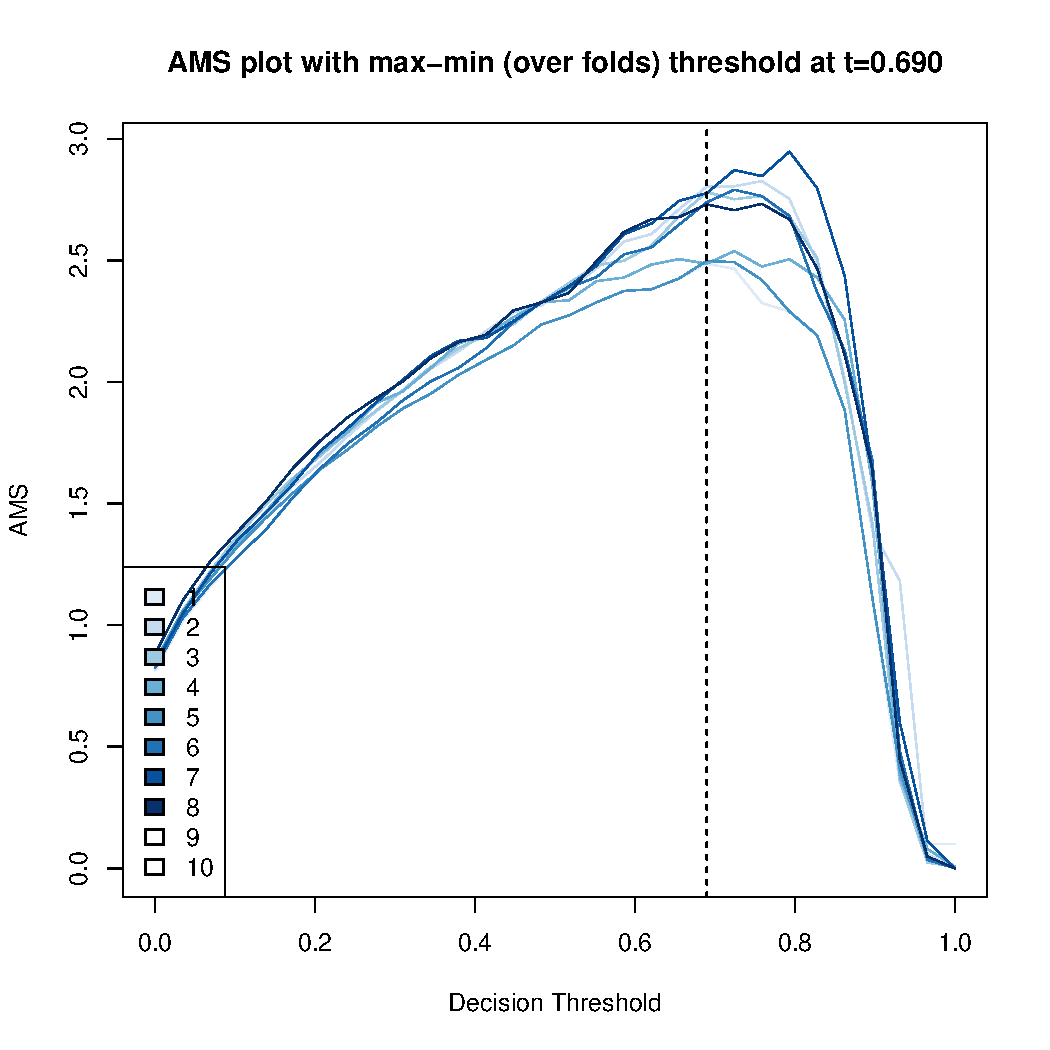
\includegraphics[width=0.4\textwidth] {cvoos-ams-curves1.pdf}
        \label{fig:ams1} } \hspace*{-0.9em}
    \subfloat[$j=1$]{
        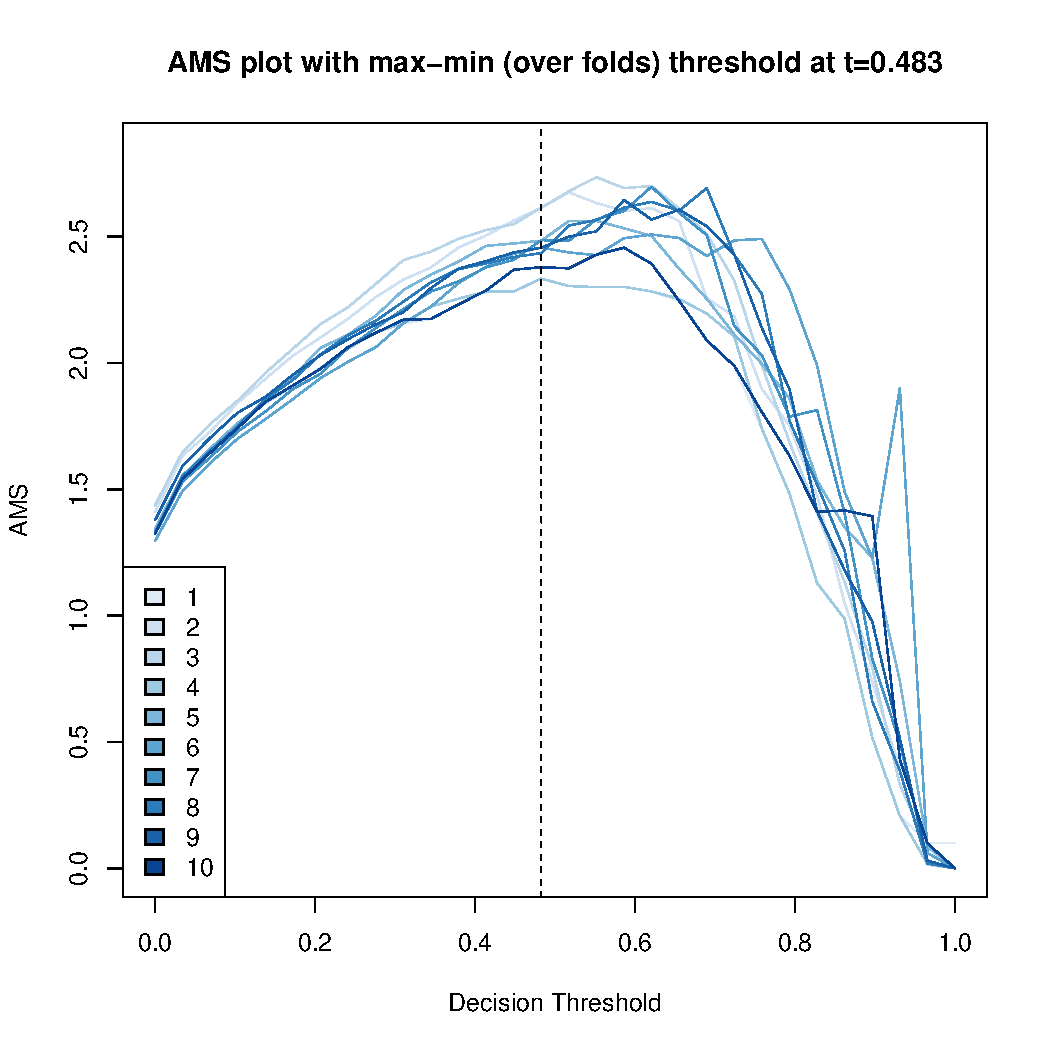
\includegraphics[width=0.4\textwidth] {cvoos-ams-curves2.pdf}
        \label{fig:ams2} } \hspace*{-0.9em}
    \subfloat[$j=2+$]{
        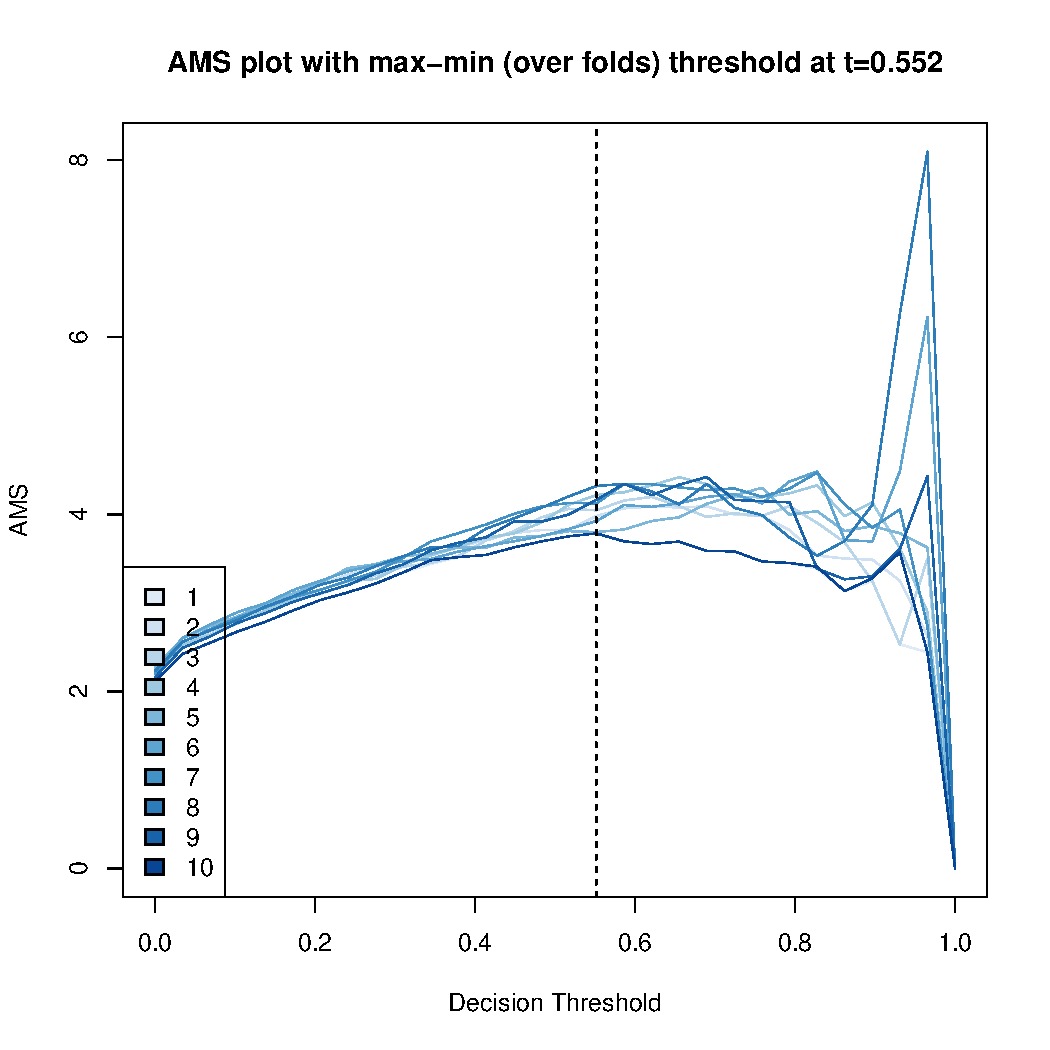
\includegraphics[width=0.4\textwidth] {cvoos-ams-curves3.pdf}
        \label{fig:ams3} }
    \end{adjustbox}
    \caption{CV OOS AMS curves for each jet category}
    \label{fig:ams_curve}
\end{figure}


\subsection{Model Selection}
To finally choose our best performing model, we needed to define the criterion with which we want to judge their success. For each experiment, we recorded both the average and mean absolute deviation of the AUC and AMS. After some consideration, we concluded that since our goal was ultimately to maximise AMS, that ought to form the primary benchmark, although experimental results show a high degree of variability between folds. As a result, we opted to scale the AMS measurements by the mean absolute deviation, to try and optimise for the most consistently effective model. The top 5 experiments according to this metric are shown in table~\ref{table:results}. 

%latex.default(output, file = path_join(c(dirname(getwd()), "doc/results_table.tex")))%
\begin{table}[!tbp]
\begin{center}
\begin{tabular}{lrrrrrrrrr}
\hline\hline
\multicolumn{1}{l}{output}&\multicolumn{1}{c}{$n_{rbf}$}&\multicolumn{1}{c}{lambda}&\multicolumn{1}{c}{poly}&\multicolumn{1}{c}{auc}&\multicolumn{1}{c}{$mad_{auc}$}&\multicolumn{1}{c}{ams}&\multicolumn{1}{c}{$mad_{ams}$}&\multicolumn{1}{c}{$scaled_{auc}$}&\multicolumn{1}{c}{$scaled_{ams}$}\tabularnewline
\hline
1&$2$&$0.000$&$3$&$0.81$&$0.063$&$1.907$&$0.855$&$12.886$&$2.230$\tabularnewline
2&$1$&$2.154$&$3$&$0.81$&$0.061$&$1.898$&$0.856$&$13.180$&$2.217$\tabularnewline
3&$2$&$2.154$&$3$&$0.81$&$0.061$&$1.898$&$0.856$&$13.180$&$2.217$\tabularnewline
4&$3$&$2.154$&$3$&$0.81$&$0.061$&$1.898$&$0.856$&$13.180$&$2.217$\tabularnewline
5&$4$&$2.154$&$3$&$0.81$&$0.061$&$1.898$&$0.856$&$13.180$&$2.217$\tabularnewline
\hline
\end{tabular}\end{center}
\end{table}


To try and determine how reliable our performance assessment might be, we plotted some figures for both performance measures (AUC and AMS) against varying regularisation, numbers of RBF centroids and order of polynomials. Restricting this summary analysis to our preferred metric, the scaled AMS, we see a noisy but somewhat consistent result in the boxplots in figure~\ref{fig:boxes}. The results for $n_{rbf}$ are particularly unclear, with a high degree of variability, whilst the polynomial results, although variable between experiments, show a decisive improvement for 2nd order polynomials. Based on these and the top experiments, we opted for a final model of the following parameters:
\eq{
    \lambda &= 1\times 10^{-4} \\
    b &= 2 \\
    n_{rbf} &= 3 \\
    \bm{\theta} &= (0.6, 0.4, 0.6)
}
for regularisation parameter $\lambda$, polynomial order $b$, number of RBF centroids $n_{rbf}$ and vector of jet group AMS thresholds $\bm{\theta} = (\theta_{j=0}, \theta_{j=1}, \theta_{j=2+})$.

\begin{figure}[htbp]
    \begin{adjustbox}{max width=1.2\linewidth,center}
    \centering
    \subfloat[$n_{rbf}$]{
        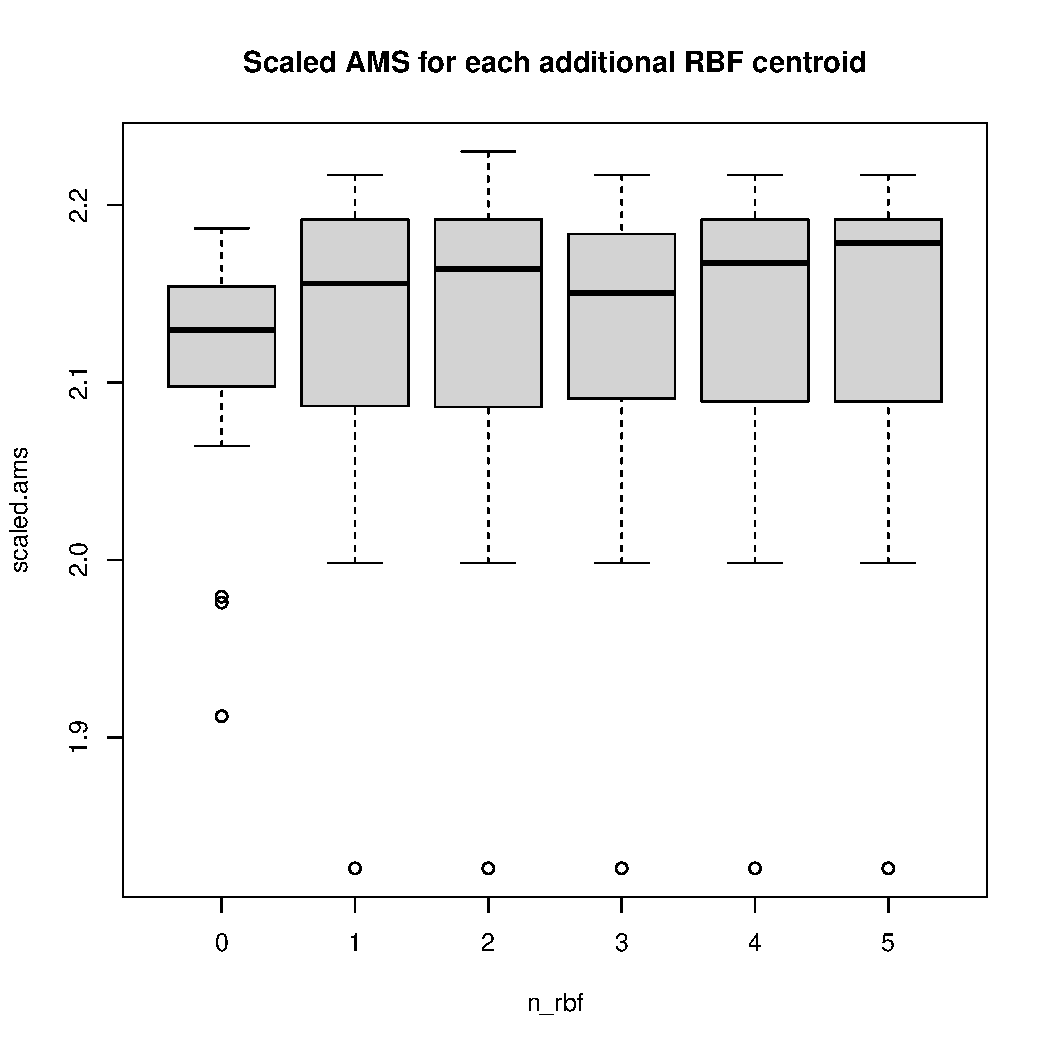
\includegraphics[width=0.4\textwidth] {boxplot-scaledams-by-nrbf.pdf}
        \label{fig:boxrbf} } \hspace*{-0.9em}
    \subfloat[Polynomial order]{
        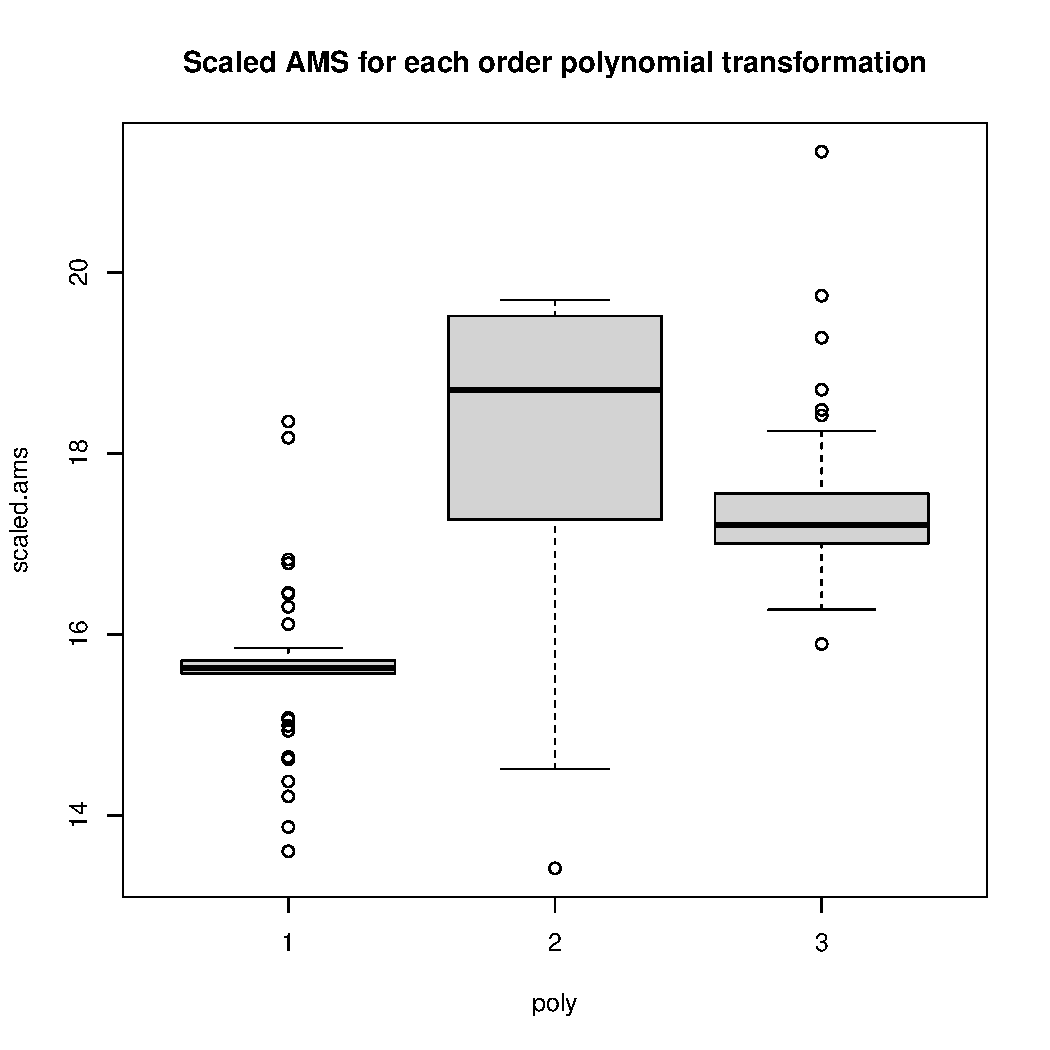
\includegraphics[width=0.4\textwidth] {boxplot-scaledams-by-poly.pdf}
        \label{fig:boxpoly} } \hspace*{-0.9em}
    \end{adjustbox}
    \caption{Box plots showing the results of experiments testing the performance of models with varying inclusion of additional features}
    \label{fig:boxes}
\end{figure}

\subsection{Predictions}
To actually calculate AMS scores, we need to convert out probabilistic outputs into binary labels which means we need to pick a decision rule, i.e. a threshold over which we assign a label 1 (or $s$) vs 0 (or $b$). Since we have a different model per jet group, we choose a different optimal threshold per model type and calculate our overall result by computing the average AMS over each group (applying its threshold) and averaging the results. Restating the same thing in more mathematical notation, we compute 
\eq{
    \langle \rm{AMS} \rangle &= \frac{1}{G}\sum_{g=1}^G\frac{1}{K}\sum_{k=1}^K \rm{ams}(g, k, \theta_g)
}
with jet groups $g$, folds $k$ and threshold for group $g$, $\theta_g$ and a function $\rm{ams}(g, k, \theta_g)$ which computes the AMS for a particular group-fold combination given its threshold.

Using the model that ranked the best in terms of scaled AMS, we get the following results on the cross-validated out-of-sample performance for the training set and the hold-out test set are in table~\ref{table:final_results}
%latex.default(output, file = path_join(c(dirname(getwd()), "doc/final_results_table.tex")),     caption = sprintf("Results for $\\lambda=%.2g$, $G=%i$, $n_{rbf}=%i$, $b=%i$, K=%i on training set (`%s') and validation set (`%s')",         lambda, G, n_rbf, poly_order, K, train_label, val_label),     label = "table:final_results")%
\begin{table}[!tbp]
\caption{Results for $\lambda=0.0001$, $G=3$, $n_{rbf}=3$, $b=2$, K=10 on training set (`t') and validation set (`v')\label{table:final_results}} 
\begin{center}
\begin{tabular}{lrrrr}
\hline\hline
\multicolumn{1}{l}{output}&\multicolumn{1}{c}{AUC}&\multicolumn{1}{c}{mad.AUC}&\multicolumn{1}{c}{AMS}&\multicolumn{1}{c}{mad.AMS}\tabularnewline
\hline
CV OOS&$0.869$&$0.01$&$3.017$&$0.168$\tabularnewline
Test set&$0.845$&$$&$2.738$&$$\tabularnewline
\hline
\end{tabular}\end{center}
\end{table}

where the ``error" term here shows the average mean absolute deviation per group across folds. 

Clearly the result for the test set is significantly worse than that for the 10-fold out-of-sample measure. A possible explanation can be found by looking at the AMS threshold curves for the two datasets for this model. For the group corresponding to 0 jets, the threshold for the maximum AMS is substantially lower than what we saw in the training set at 0.2 compared to 0.6. The other two jet categories have an optimal threshold of 0.5 in the test set, versus 0.4 and 0.6 in the training set. 

\begin{figure}[h]
    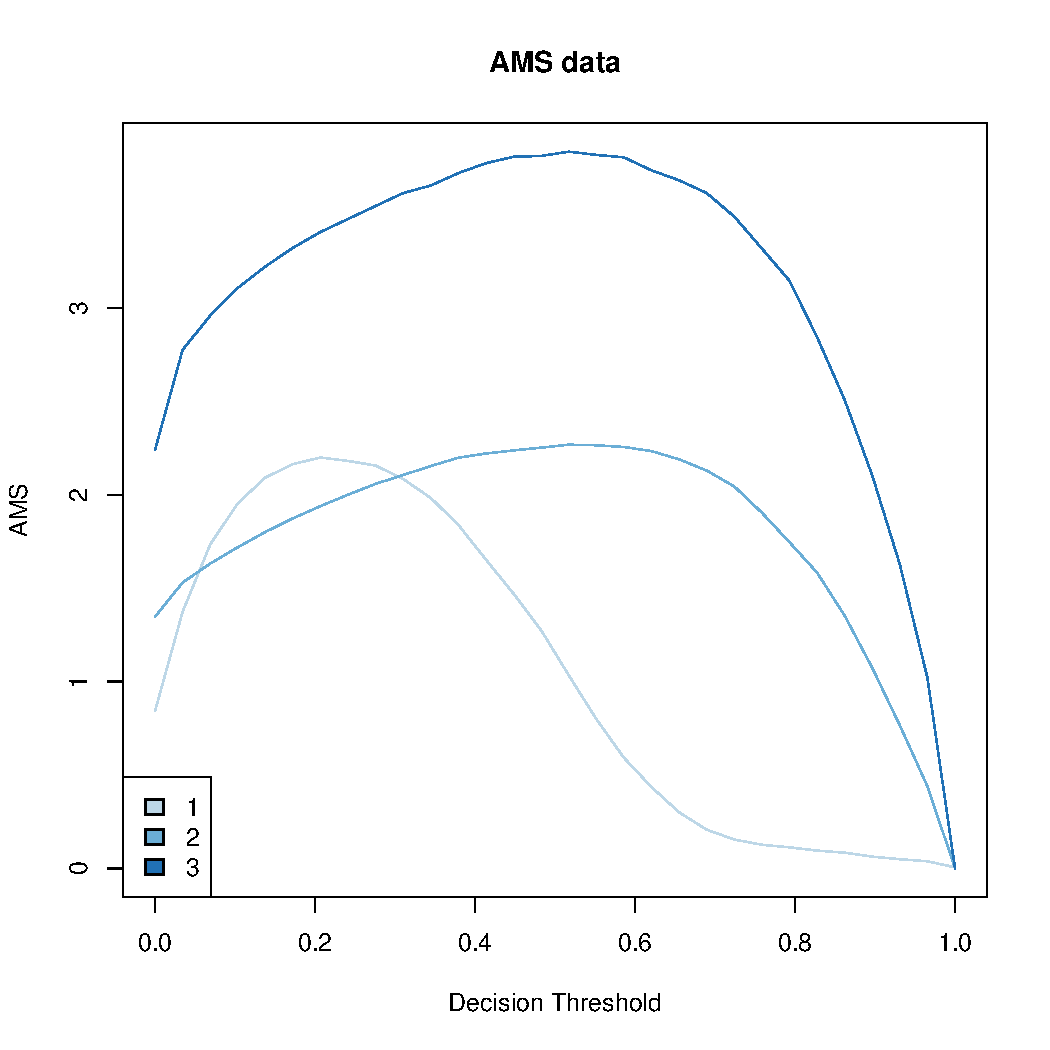
\includegraphics[width=8cm]{validation-ams-curves.pdf}
    \caption{AMS curves for the test set}
\end{figure}

\section{Conclusion}
\label{conclusion}


\pagebreak 


\begin{appendices}
\section{AMS}
\label{appendix:ams}
Is the AMS metric convex?
\eq{
    \rm{AMS} &= \sqrt{2\left((s+b)\log(1+\frac{s}{b})-s\right)}
}

In the documentation, the implication is that in general, we expect $b \gg s$ giving the approximate AMS as $\rm{AMS} \sim \frac{s}{\sqrt{b}}(1+\mc{O}(\frac{s}{b}))$.

If we directly check the derivatives of the approximate AMS in the large $b$ regime:
\eq{
    \pd_s^2\frac{s}{\sqrt{b}} &= 0\\
    \pd_b^2\frac{s}{\sqrt{b}} &= \frac{3}{4}\frac{s}{b^{5/2}} >0\\
    \pd_{bs}^2 &= -\frac{1}{2b^{3/2}} < 0
}
which implies non-convexity (and non-concavity).

To check more carefully though, calculate the terms of the Hessian of the original and then apply the approximation:
\eq{
    \pd_s\rm{AMS} &= \rm{AMS}^{-1}\log\left(1+\frac{s}{b}\right) \\
    \pd_b\rm{AMS} &= \rm{AMS}^{-1}\left(\log(1+\frac{s}{b}) -\frac{s}{b}\right) \\
    \pd_s^2\rm{AMS} &= \rm{AMS}^{-1}\left(\frac{1}{b+s} - \rm{AMS}^{-2}\log(1+\frac{s}{b})^2\right) \\
    \pd_b^2\rm{AMS} &= \rm{AMS}^{-1}\left(\frac{s^2}{b^2(s+b)} -\rm{AMS}^{-2}(\log(1+\frac{s}{b}) -\frac{s}{b})^2\right) \\
    \pd_{sb}^2\rm{AMS} &= -\rm{AMS}^{-1}\left(\frac{s}{b(s+b)} - \rm{AMS}^{-2}\log(1+\frac{s}{b})(\log(1+\frac{s}{b}) -\frac{s}{b})\right)
}
and then verify whether any of them are ever $<0$.

Using the AMS approximation, and $\log\left(1+\frac{s}{b}\right) \sim \frac{s}{b} - \half\left(\frac{s}{b}\right)^2$ we get the following
\eq{
    \pd_s^2\rm{AMS} &\sim \frac{\sqrt{b}}{s}\left[\frac{1}{(b+s)} - \frac{b}{s^2}(\frac{s^2}{b^2} - \frac{s^3}{b^3})\right] \\
    &= \frac{\sqrt{b}}{s(s+b)} - \frac{1}{s\sqrt{b}} + \frac{1}{b^{3/2}} \\
    &\gtrsim \eps
}
Since in this regime of large $b$ this term is negative, the Hessian cannot be positive definite and hence the metric is non-convex. If the Hessian is \emph{concave} though, we can simply optimize $-\rm{AMS}$, so we need to check the other terms.

\eq{
    \pd_b^2\rm{AMS} &\sim \frac{\sqrt{b}}{s}\left[\frac{s^2}{b^2(s+b)} - \frac{b}{s^2}(\frac{1}{4}\frac{s^4}{b^4})\right] \\
    &= \frac{s}{b^{3/2}(s+b)} - \frac{1}{4}\frac{s}{b^{5/2}} \\
    &\gtrsim \eps
}

\eq{
    \pd_{bs}^2\rm{AMS} &\sim -\frac{\sqrt{b}}{s}\left[\frac{s}{b(s+b)} + \frac{b}{s^2}(\frac{s}{b} -\half\frac{s}{b^2})(-\half\frac{s^2}{b^2})\right] \\
    &= \frac{1}{2b^{3/2}}(1-\half s) - \frac{1}{\sqrt{b}(s+b)} \\
    &< 0
}

where we take $\eps$ to be some suitably small positive number.

If we decide to take some tolerance, $\eps \sim 10^{-6}$ at which to ignore higher order terms in $\frac{s}{b}$ we can check specifically that the claims on the Hessian above hold in that regime.

So, let's assume we can ignore terms of $O(\frac{s}{b})^3$ then for $\eps\sim 10^{-6}$ a ratio of $\frac{s}{b}\sim 10^{-2}$ would suffice; so to test this, let us choose $s=1$ and $b=100$ for simplicity.
With this, we find that $\pd_s^2\rm{AMS} \sim +10^{-6}$, $\pd_b^2\rm{AMS} \sim +10^{-6}$ and $\pd_{bs}^2\rm{AMS} \sim -10^{-4}$ which satisfies the claims above.
Finally, to verify that this is a reasonable assertion, if we check the ratio of $s:b$ in the data (using the weight vector) we find a ratio of approximately $10^{-3}$, which means our assumption was conservative. 


\section{Modelling}

\subsection{Newton's Method for Logistic Regression}
\label{appendix:newton_lr}
From the conditional distribution under the logistic regression model for a single point $\xv \in R^d$, $y \in \{+1,-1\}$ and coefficients $\betav \in R^d$.
\eq{
    p(y\given \xv, \betav) &= \sigma(f(\xv;\betav)\cdot y) \\
    &= (1 + \exp(y\inprod{\xv}{\betav}))^{-1}
}

We want to minimise the negative loglikelihood:
\eq{
    l(\xv, y, \betav) &= \log(1 + \e^{y\inprod{\xv}{\xv}}) \\
    \pd_{\beta_a} l &= \frac{yx_a\e^{y\inprod{\xv}{\betav}}}{1 + \e^{y\inprod{\xv}{\betav}}} \\
    \pd^2_{\beta_a \beta_b}l &= \frac{y^2x_ax_b\e^{y\inprod{\xv}{\betav}}}{(1+\e^{y\inprod{\xv}{\betav}})^2}\left( 1 + \e^{y\inprod{\xv}{\betav}} - \e^{y\inprod{\xv}{\betav}}\right) \\
    &= \frac{x_ax_b\e^{y\inprod{\xv}{\betav}}}{(1+\e^{y\inprod{\xv}{\betav}})^2}\\
    &= x_ax_bw(x)
}
where in the last line we define a weight function $w(x) = \frac{\e^{-x}}{(1+\e^{-x})^2}$ (and the elementwise vector version, $\wv(\xv) = \frac{\e^{-\xv}}{(1+\e^{-\xv})^2}$).

To implement Newton's method we want to try and simplify the expressions. First define the logistic and logit functions as
\eq{
    \gamma(x) &= (1+\e^{-x})^{-1} \\
    \gamma^{-1}(p) &= \log\left(\frac{p}{1-p}\right)
}
and then write out the derivatives in terms of the logistic function:
\eq{
    \pd_{\beta_a} l(y=+1) &= x_a\gamma(\inprod{\xv}{\betav}) \\
    \pd_{\beta_a} l(y=-1) &= -x_a(1-\gamma(\inprod{\xv}{\betav})
}
If we then map $y \in \{1,-1\}$ to $y' \in \{0,1\}$ we can condense these into a single expression
\eq{
    \pd_{\beta_a} l(y) &= -x_a(y - \gamma(\inprod{\xv}{\betav}))
}
and rewrite the loss as $l(y') = \log(1+\e^{(-1)^{y'}\inprod{\xv}{\betav}})$.

Now for our entire dataset $D$, assumed to be IID, we have a total loss, gradient and Hessian
\eq{
    L &= \sum_{i \in D}l_i = \sum_{i \in D}\log(1+\e^{y_i\inprod{\xv_i}{\betav}})\\
    \pd_{\betav}L &= -\sum_{i \in D}\xv_i(y_i - \gamma(\inprod{\xv_i}{\betav})) \\
    &= -\Xv^T(\yv-\gamma(\Xv\betav)) \\
    \bm{H} &= \sum_{i \in D}\xv_i\xv_i^Tw(\xv_i)\\
    &= \Xv^T\bm{W}\Xv
}
with $\Xv = \bp \xv_1^T \\ \vdots \\ \xv_n^T \ep \in R^{n\times d}$, $\bm{W} = \diag(\wv(\xv)) \in R^{n\times n}$.

\subsubsection{Regularisation}
We can add constraints to our minimisation problem, to help constrain the coefficients and effectively implement $L_2$ regularisation by formulating the following convex optimisation problem.
\eq{
    \min. &\quad L \\
    \st &\quad \norm{\betav}^2\leq c
}
From this we can construct the Lagrangian $\mc{L} = L + \lambda(\norm{\betav}^2 - c)$ and hence augment the gradient and Hessian we calculated above as
\eq{
    \pd_{\betav}\mc{L} &= \pd_{\betav}L + 2\lambda\betav \\
    \bm{\tilde{H}} &= \bm{H} + 2\lambda\Iv
}

Since we have a free parameter $c$ that determines the optimal value $\lambda^\star(c)$ of our dual variable, we can equivalently ignore $c$ and treat $\lambda$ as a parameter to be tuned.

\subsubsection{Newton's method}

\begin{algorithm}[H]
    1. Initialise parameters; $\betav_0$, $\lambda_0$, $\eps$, $L_0 = L(\betav_0)$, $m$\\
    2. \For{i=1:m}{
        Compute $\pd_{\betav}L$ and $\bm{H}$\\
        Calculate Newton step $\Delta\betav = -\bm{H}^{-1}\pd_{\betav}L$\\
        Calculate stepsize $\alpha$ with backtracking linesearch (\ref{algo:line}) \\
        Update $\betav \leftarrow \betav + \alpha\Delta\betav$ \\
        Compute new loss $L$ \\
        Test stopping criterion: $|L-L_0| < \eps$
    } 
    3. Return $\hat{\betav}$.\\
    \caption{Newton's method}
\end{algorithm}
\label{algo:newton}

\begin{algorithm}[H]
    1. Initialise parameters; $\gamma, \tau$ \\
    2. Set largest stepsize $s_{max}\leftarrow 1$ \\
    3. Set $s \leftarrow s_{max}$ \\
    4. \While{$f(x+\Delta x) > f(x) + \gamma s \nabla f^T\Delta x$} {
        Update $s\leftarrow \tau s$ \\
    }
    5. Return $s$
    \caption{Backtracking linesearch}
\end{algorithm}
\label{algo:line}

\end{appendices}
\bibliography{lhc.bib}{}
\bibliographystyle{plain}

\end{document}